\documentclass[10pt,oneside]{article}
\usepackage[T1]{fontenc}
\usepackage[utf8]{inputenc}
% \usepackage{lmodern}
%\usepackage[adobe-utopia,uppercase=upright,greeklowercase=upright]{mathdesign}
\usepackage[adobe-utopia]{mathdesign}
%\usepackage{minionpro}
% \usepackage{pifont}
% \usepackage{amssymb}
\usepackage{amsmath}
\usepackage[francais]{babel}
% \usepackage[francais]{varioref}
\usepackage[dvips]{graphicx}

\usepackage{framed}
\usepackage[normalem]{ulem}
\usepackage{fancyhdr}
\usepackage{titlesec}
\usepackage{vmargin}
\usepackage{longtable}

\usepackage{ifthen}


%\usepackage{epsfig}
\usepackage{subfig}

\usepackage{multirow}
\usepackage{multicol} % Portions de texte en colonnes
\usepackage{flafter}%floatants après la référence



\usepackage{color}
\usepackage{colortbl}


\definecolor{gris25}{gray}{0.75}
\definecolor{bleu}{RGB}{18,33,98}
\definecolor{bleuf}{RGB}{42,94,171}
\definecolor{bleuc}{RGB}{231,239,247}
\definecolor{rougef}{RGB}{185,18,27}
\definecolor{rougec}{RGB}{255,230,231}
\definecolor{vertf}{RGB}{103,126,82}
\definecolor{vertc}{RGB}{220,255,191}
\definecolor{violetf}{RGB}{112,48,160}
\definecolor{violetc}{RGB}{230,224,236}

\newenvironment{sci}[1][\hsize]%
{%
    \def\FrameCommand%
    {%
%\rotatebox{90}{\textit{\textsf{Scilab}}\includegraphics[height=.8cm]{png/logo_scilab}} 
\rotatebox{90}{\includegraphics[height=.6cm]{png/logo_scilab}} 
        {\color{violetf}\vrule width 3pt}%
        \hspace{0pt}%must no space.
        \fboxsep=\FrameSep\colorbox{violetc}%
    }%
    \MakeFramed{\hsize #1 \advance\hsize-\width\FrameRestore}%
}%
{\endMakeFramed}%

\newenvironment{pseudo}[1][\hsize]%
{%
    \def\FrameCommand%
    {%
\rotatebox{90}{\textit{\textsf{Pseudo Code}}} 
        {\color{violetf}\vrule width 3pt}%
        \hspace{0pt}%must no space.
        \fboxsep=\FrameSep\colorbox{violetc}%
    }%
    \MakeFramed{\hsize #1 \advance\hsize-\width\FrameRestore}%
}%
{\endMakeFramed}%

\newenvironment{py}[1][\hsize]%
{%
    \def\FrameCommand%
    {%
%\rotatebox{90}{\textit{\textsf{Python}}} 
\rotatebox{90}{\includegraphics[height=.6cm]{png/logo_python}} 
        {\color{violetf}\vrule width 3pt}%
        \hspace{0pt}%must no space.
        \fboxsep=\FrameSep\colorbox{violetc}%
    }%
    \MakeFramed{\hsize #1 \advance\hsize-\width\FrameRestore}%
}%
{\endMakeFramed}%


\newenvironment{corrige}[1][\hsize]%
{%
    \def\FrameCommand
    {%
\rotatebox{90}{\textit{\textsf{Correction}}} 
        {\color{violetf}\vrule width 3pt}%
        \hspace{0pt}%must no space.
        \fboxsep=\FrameSep\colorbox{violetc}%
    }%
    \MakeFramed{\hsize#1\advance\hsize-\width\FrameRestore}%
}%
{\endMakeFramed}%



\newenvironment{rem}[1][\hsize]%
{%
    \def\FrameCommand
    {%
\rotatebox{90}{\textit{\textsf{Remarque}}} 
        {\color{bleuf}\vrule width 3pt}%
        \hspace{0pt}%must no space.
        \fboxsep=\FrameSep\colorbox{bleuc}%
    }%
    \MakeFramed{\hsize#1\advance\hsize-\width\FrameRestore}%
}%
{\endMakeFramed}%


\newenvironment{savoir}[1][\hsize]%
{%
    \def\FrameCommand
    {%
\rotatebox{90}{\textit{\textsf{Savoir}}} 
        {\color{bleuf}\vrule width 3pt}%
        \hspace{0pt}%must no space.
        \fboxsep=\FrameSep\colorbox{bleuc}%
    }%
    \MakeFramed{\hsize#1\advance\hsize-\width\FrameRestore}%
}%
{\endMakeFramed}%

\newenvironment{prob}[1][\hsize]%
{%
    \def\FrameCommand%
    {%
\rotatebox{90}{\textit{\textsf{ Problématique}}} 
        {\color{rougef}\vrule width 3pt}%
        \hspace{0pt}%must no space.
        \fboxsep=\FrameSep\colorbox{rougec}%
    }%
    \MakeFramed{\hsize#1\advance\hsize-\width\FrameRestore}%
}%
{\endMakeFramed}%

\newenvironment{obj}[1][\hsize]%
{%
    \def\FrameCommand%
    {%
\rotatebox{90}{\textit{\textsf{ $\;$}}} 
        {\color{rougef}\vrule width 3pt}%
        \hspace{0pt}%must no space.
        \fboxsep=\FrameSep\colorbox{rougec}%
    }%
    \MakeFramed{\hsize#1\advance\hsize-\width\FrameRestore}%
}%
{\endMakeFramed}%

\newenvironment{defi}[1][\hsize]%
{%
    \def\FrameCommand%
    {%
\rotatebox{90}{\textit{\textsf{Définition\\}}} 
        {\color{bleuf}\vrule width 3pt}%
        \hspace{0pt}%must no space.
        \fboxsep=\FrameSep\colorbox{bleuc}%
    }%
    \MakeFramed{\hsize#1\advance\hsize-\width\FrameRestore}%
}%
{\endMakeFramed}%


\newenvironment{demo}[1][\hsize]%
{%
    \def\FrameCommand%
    {%
\rotatebox{90}{\textit{\textsf{Démonstration\\}}} 
        {\color{bleuf}\vrule width 3pt}%
        \hspace{0pt}%must no space.
        \fboxsep=\FrameSep\colorbox{bleuc}%
    }%
    \MakeFramed{\hsize#1\advance\hsize-\width\FrameRestore}%
}%
{\endMakeFramed}%


\newenvironment{hypo}[1][\hsize]%
{%
    \def\FrameCommand%
    {%
\rotatebox{90}{\textit{\textsf{Hypothèse\\}}} 
        {\color{bleuf}\vrule width 3pt}%
        \hspace{0pt}%must no space.
        \fboxsep=\FrameSep\colorbox{bleuc}%
    }%
    \MakeFramed{\hsize#1\advance\hsize-\width\FrameRestore}%
}%
{\endMakeFramed}%


\newenvironment{prop}[1][\hsize]%
{%
    \def\FrameCommand%
    {%
\rotatebox{90}{\textit{\textsf{Propriété\\}}} 
        {\color{bleuf}\vrule width 3pt}%
        \hspace{0pt}%must no space.
        \fboxsep=\FrameSep\colorbox{bleuc}%
    }%
    \MakeFramed{\hsize#1\advance\hsize-\width\FrameRestore}%
}%
{\endMakeFramed}%

\newenvironment{props}[1][\hsize]%
{%
    \def\FrameCommand%
    {%
\rotatebox{90}{\textit{\textsf{Propriétés\\}}} 
        {\color{bleuf}\vrule width 3pt}%
        \hspace{0pt}%must no space.
        \fboxsep=\FrameSep\colorbox{bleuc}%
    }%
    \MakeFramed{\hsize#1\advance\hsize-\width\FrameRestore}%
}%
{\endMakeFramed}%

\newenvironment{exemple}[1][\hsize]%
{%
    \def\FrameCommand%
    {%
\rotatebox{90}{\textit{\textsf{Exemple\\}}} 
        {\color{vertf}\vrule width 3pt}%
        \hspace{0pt}%must no space.
        \fboxsep=\FrameSep\colorbox{vertc}%
    }%
    \MakeFramed{\hsize#1\advance\hsize-\width\FrameRestore}%
}%
{\endMakeFramed}%

\newenvironment{resultat}[1][\hsize]%
{%
    \def\FrameCommand%
    {%
\rotatebox{90}{\textit{\textsf{Résultat\\}}} 
        {\color{rougef}\vrule width 3pt}%
        \hspace{0pt}%must no space.
        \fboxsep=\FrameSep\colorbox{rougec}%
    }%
    \MakeFramed{\hsize#1\advance\hsize-\width\FrameRestore}%
}%
{\endMakeFramed}%

\newenvironment{methode}[1][\hsize]%
{%
    \def\FrameCommand%
    {%
\rotatebox{90}{\textit{\textsf{Méthode\\}}} 
        {\color{rougef}\vrule width 3pt}%
        \hspace{0pt}%must no space.
        \fboxsep=\FrameSep\colorbox{rougec}%
    }%
    \MakeFramed{\hsize#1\advance\hsize-\width\FrameRestore}%
}%
{\endMakeFramed}%

\newenvironment{theo}[1][\hsize]%
{%
    \def\FrameCommand%
    {%
\rotatebox{90}{\textit{\textsf{Théorème\\}}} 
        {\color{rougef}\vrule width 3pt}%
        \hspace{0pt}%must no space.
        \fboxsep=\FrameSep\colorbox{rougec}%
    }%
    \MakeFramed{\hsize#1\advance\hsize-\width\FrameRestore}%
}%
{\endMakeFramed}%

\newenvironment{warn}[1][\hsize]%
{%
    \def\FrameCommand%
    {%
\rotatebox{90}{\textit{\textsf{Attention\\}}} 
        {\color{rougef}\vrule width 3pt}%
        \hspace{0pt}%must no space.
        \fboxsep=\FrameSep\colorbox{rougec}%
    }%
    \MakeFramed{\hsize#1\advance\hsize-\width\FrameRestore}%
}%
{\endMakeFramed}%

% \usepackage{pstricks}
%\usepackage{minitoc}
% \setcounter{minitocdepth}{4}

\setcounter{tocdepth}{2}

% \mtcselectlanguage{french} 

%\usepackage{draftcopy}% "Brouillon"
% \usepackage{floatflt}
\usepackage{psfrag}
%\usepackage{listings} % Permet d'insérer du code de programmation
\renewcommand{\baselinestretch}{1.2}

% Changer la numérotation des figures :
% ------------------------------------
% \makeatletter
% \renewcommand{\thefigure}{\ifnum \c@section>\z@ \thesection.\fi
%  \@arabic\c@figure}
% \@addtoreset{figure}{section}
% \makeatother
 


%%%%%%%%%%%%
% Définition des vecteurs %
%%%%%%%%%%%%
 \newcommand{\vect}[1]{\overrightarrow{#1}}

%%%%%%%%%%%%
% Définition des torseusr %
%%%%%%%%%%%%

 \newcommand{\torseur}[1]{%
\left\{{#1}\right\}
}

\newcommand{\torseurcin}[3]{%
\left\{\mathcal{#1} \left(#2/#3 \right) \right\}
}

\newcommand{\torseurstat}[3]{%
\left\{\mathcal{#1} \left(#2\rightarrow #3 \right) \right\}
}

 \newcommand{\torseurc}[8]{%
%\left\{#1 \right\}=
\left\{
{#1}
\right\}
 = 
\left\{%
\begin{array}{cc}%
{#2} & {#5}\\%
{#3} & {#6}\\%
{#4} & {#7}\\%
\end{array}%
\right\}_{#8}%
}

 \newcommand{\torseurcol}[7]{
\left\{%
\begin{array}{cc}%
{#1} & {#4}\\%
{#2} & {#5}\\%
{#3} & {#6}\\%
\end{array}%
\right\}_{#7}%
}

 \newcommand{\torseurl}[3]{%
%\left\{\mathcal{#1}\right\}_{#2}=%
\left\{%
\begin{array}{l}%
{#1} \\%
{#2} %
\end{array}%
\right\}_{#3}%
}

 \newcommand{\vectv}[3]{%
\vect{V\left( {#1} \in {#2}/{#3}\right)}
}


\newcommand{\vectf}[2]{%
\vect{R\left( {#1} \rightarrow {#2}\right)}
}

\newcommand{\vectm}[3]{%
\vect{\mathcal{M}\left( {#1}, {#2} \rightarrow {#3}\right)}
}


 \newcommand{\vectg}[3]{%
\vect{\Gamma \left( {#1} \in {#2}/{#3}\right)}
}

 \newcommand{\vecto}[2]{%
\vect{\Omega\left( {#1}/{#2}\right)}
}
% }$$\left\{\mathcal{#1} \right\}_{#2} =%
% \left\{%
% \begin{array}{c}%
%  #3 \\%
%  #4 %
% \end{array}%
% \right\}_{#5}}

%  ------------------------------------------
% | Modification du formatage des sections : | 
%  ------------------------------------------

% Grands titres :
% ---------------

\newcommand{\titre}[1]{%
\begin{center}
      \bigskip
      \rule{\textwidth}{1pt}
      \par\vspace{0.1cm}
      
      \textbf{\large #1}
      \par\rule{\textwidth}{1pt}
    \end{center}
    \bigskip
  }

% Supprime le numéro du chapitre dans la numérotation des sections:
% -----------------------------------------------------------------
\makeatletter
\renewcommand{\thesection}{\@arabic\c@section}
\makeatother


% \titleformat{\chapter}[display]
% {\normalfont\Large\filcenter}
% {}
% {1pc}
% {\titlerule[1pt]
%   \vspace{1pc}%
%   \Huge}[\vspace{1ex}%
% \titlerule]


%%%% Chapitres Comme PY Pechard %%%%%%%%%
% numéro du chapitre
\DeclareFixedFont{\chapnumfont}{OT1}{phv}{b}{n}{80pt}
% pour le mot « Chapitre »
\DeclareFixedFont{\chapchapfont}{OT1}{phv}{m}{it}{40pt}
% pour le titre
\DeclareFixedFont{\chaptitfont}{T1}{phv}{b}{n}{25pt}

\definecolor{gris}{gray}{0.75}
\titleformat{\chapter}[display]%
	{\sffamily}%
	{\filleft\chapchapfont\color{gris}\chaptertitlename\
	\\
	\vspace{12pt}
	\chapnumfont\thechapter}%
	{16pt}%
	{\filleft\chaptitfont}%
	[\vspace{6pt}\titlerule\titlerule\titlerule]

%%%%  Fin Chapitres Comme PY Pechard %%%%%%%%%


% Section, subsection, subsubsection sans serifs :
% % ----------------------------------------------

% \makeatletter
% \renewcommand{\section}{\@startsection{section}{0}{0mm}%
% {\baselineskip}{.3\baselineskip}%
% {\normalfont\sffamily\Large\textbf}}%
% \makeatother

\makeatletter
\renewcommand{\@seccntformat}[1]{{\textcolor{bleu}{\csname
the#1\endcsname}\hspace{0.5em}}}
\makeatother

\makeatletter
\renewcommand{\section}{\@startsection{section}{1}{\z@}%
                       {-4ex \@plus -1ex \@minus -.4ex}%
                       {1ex \@plus.2ex }%
                       {\normalfont\Large\sffamily\bfseries}}%
\makeatother
 
\makeatletter
\renewcommand{\subsection}{\@startsection {subsection}{2}{\z@}
                          {-3ex \@plus -0.1ex \@minus -.4ex}%
                          {0.5ex \@plus.2ex }%
                          {\normalfont\large\sffamily\bfseries}}
\makeatother
 
\makeatletter
\renewcommand{\subsubsection}{\@startsection {subsubsection}{3}{\z@}
                          {-2ex \@plus -0.1ex \@minus -.2ex}%
                          {0.2ex \@plus.2ex }%
                          {\normalfont\large\sffamily\bfseries}}
\makeatother
 
\makeatletter             
\renewcommand{\paragraph}{\@startsection{paragraph}{4}{\z@}%
                                    {-2ex \@plus-.2ex \@minus .2ex}%
                                    {0.1ex}%               
{\normalfont\sffamily\bfseries}}
\makeatother
 

\makeatletter             
\renewcommand{\subparagraph}{\@startsection{subparagraph}{5}{\z@}%
                                    {-2ex \@plus-.2ex \@minus .2ex}%
                                    {0.1ex}%               
{\normalfont\bfseries Question }}
\makeatother

\renewcommand{\thesubparagraph}{\arabic{subparagraph}} 
%
\makeatletter
%\renewcommand{\subparagraph}{\@startsection{subparagraph}{5}{\z@}%
%                                       {-2ex \@plus-.1ex \@minus .2ex}%
%                                       {0.1ex}%
%				    {\normalfont\normalsize\sffamily\bfseries}}
%\makeatletter
% \makeatletter
% \renewcommand{\subsection}{\@startsection{subsection}{1}{2mm}%
% {\baselineskip}{.3\baselineskip}%
% {\normalfont\sffamily\large\textbf}}%
% \makeatother
% 
% \makeatletter
% \renewcommand{\subsubsection}{\@startsection{subsubsection}{2}{4mm}%
% {\baselineskip}{.15\baselineskip}%
% {\normalfont\sffamily\large\textbf}}%
% \makeatother
% 
% \makeatletter
% \renewcommand{\paragraph}{\@startsection{paragraph}{3}{6mm}%
% {\baselineskip}{.15\baselineskip}%
% {\normalfont\sffamily\large\textbf}}%
% \makeatother
 
\setcounter{secnumdepth}{5}


%  --------
% | Marges |
%  --------


% \setmarginsrb{2.5cm}{1.5cm}{2.5cm}{2cm}{1cm}{1cm}{1cm}{1cm}
\setmarginsrb{1.5cm}{1cm}{1cm}{1.5cm}{1cm}{1cm}{1cm}{1cm}

% Changer les marges localement :
% -----------------------------
\newenvironment{changemargin}[2]{\begin{list}{}{%
\setlength{\topsep}{0pt}%
\setlength{\leftmargin}{0pt}%
\setlength{\rightmargin}{0pt}%
\setlength{\listparindent}{\parindent}%
\setlength{\itemindent}{\parindent}%
\setlength{\parsep}{0pt plus 1pt}%
\addtolength{\leftmargin}{#1}%
\addtolength{\rightmargin}{#2}%
}\item }{\end{list}}



\usepackage{pst-solides3d}
\usepackage{titletoc}
\titlecontents{chapter}[+3pc]
  {\addvspace{10pt}\sffamily\bfseries}
{\contentslabel[{\pscirclebox[fillstyle=solid,fillcolor=gray!25,
linecolor=gray!25,framesep=4pt]{\textcolor{white}{\thecontentslabel}}}]{2.5pc}}
  {}
  {\dotfill \normalfont\thecontentspage\ }

\titlecontents{section}[3pc]
  {\addvspace{2pt}\sffamily}
  {\contentslabel[\thecontentslabel]{1.8pc}}
  {}
  {\dotfill \normalfont\thecontentspage\ }

\titlecontents{subsection}[5pc]
  {\addvspace{2pt}\sffamily}
  {\contentslabel[\thecontentslabel]{1.8pc}}
  {}
  {\dotfill \normalfont\thecontentspage\ }

\titlecontents{subsubsection}[8pc]
  {\addvspace{2pt}\sffamily}
  {\contentslabel[\thecontentslabel]{3pc}}
  {}
  {\dotfill \normalfont\thecontentspage\ }
%{\;\titlerule\;\normalfont\thecontentspage\ }

\titlecontents{paragraph}[9pc]
  {\addvspace{2pt}\sffamily}
  {\contentslabel[\thecontentslabel]{3.5pc}}
  {}
  {\dotfill \normalfont\thecontentspage\ }





%Si le boolen xp est vrai : compilation pour xabi
%Sinon compilation Damien
\newboolean{xp}
\setboolean{xp}{true}

\newboolean{prof}
\setboolean{prof}{true}

\def\xxtitre{\ifthenelse{\boolean{xp}}{
CI 3 -- CIN : Étude du comportement cinématique des systèmes}{
}}

\def\xxsoustitre{\ifthenelse{\boolean{xp}}{
Chapitre 5 -- Cinématique du solide indéformable}{
}}


\def\xxauteur{\ifthenelse{\boolean{xp}}{
\noindent 2013 -- 2014 \\
Xavier \textsc{Pessoles}}{
}}


\def\xxpied{\ifthenelse{\boolean{xp}}{
CI 3 : CIN -- Cours \\
Ch 4 : Cinématique du solide -- \ifthenelse{\boolean{prof}}{P}{E}%
}{
}}

\usepackage[%
    pdftitle={CIN : Cinématique du solide},
    pdfauthor={Xavier Pessoles},
    colorlinks=true,
    linkcolor=blue,
    citecolor=magenta]{hyperref}


\usepackage{pifont}
\sloppy
\hyphenpenalty 10000


\begin{document}






% \makeatletter \let\ps@plain\ps@empty \makeatother
%% DEBUT DU DOCUMENT
%% =================




%------------- En tetes et Pieds de Pages ------------


\pagestyle{fancy}
\ifthenelse{\boolean{xp}}{%
\renewcommand{\headrulewidth}{0pt}}{%
\renewcommand{\headrulewidth}{0.2pt}} %pour mettre le trait en haut
%\renewcommand{\headrulewidth}{0.2pt}

\fancyhead{}
\fancyhead[L]{%
\ifthenelse{\boolean{xp}}{%
\noindent\begin{minipage}[c]{2.6cm}%

\includegraphics[width=2cm]{png/logo_ptsi.png}%
\end{minipage}%
}{%
\footnotesize{\textit{\textsf{Lycée François Premier}}}
}}

\ifthenelse{\boolean{xp}}{%
\fancyhead[C]{\rule{12cm}{.5pt}}}{
}


\fancyhead[R]{%
\noindent\begin{minipage}[c]{3cm}
\begin{flushright}
\footnotesize{\textit{\textsf{Sciences Industrielles \\ de l'ingénieur}}}%
\end{flushright}
\end{minipage}
}


\ifthenelse{\boolean{xp}}{%
\fancyhead[C]{\rule{12cm}{.5pt}}}{
}

\renewcommand{\footrulewidth}{0.2pt}

\fancyfoot[C]{\footnotesize{\bfseries \thepage}}
\fancyfoot[L]{%
\begin{minipage}[c]{.2\linewidth}
\noindent\footnotesize{{\xxauteur}}
\end{minipage}
\ifthenelse{\boolean{xp}}{}{%
\begin{minipage}[c]{.15\linewidth}
\includegraphics[width=2cm]{png/logoCC.png}
\end{minipage}}
}


\fancyfoot[R]{\footnotesize{\xxpied}}



\begin{center}
 \huge\textsc{\xxtitre}

\end{center}

\begin{center}
 \LARGE\textsc{\xxsoustitre}
\end{center}


\begin{minipage}[c]{.3\linewidth}
\begin{center}
%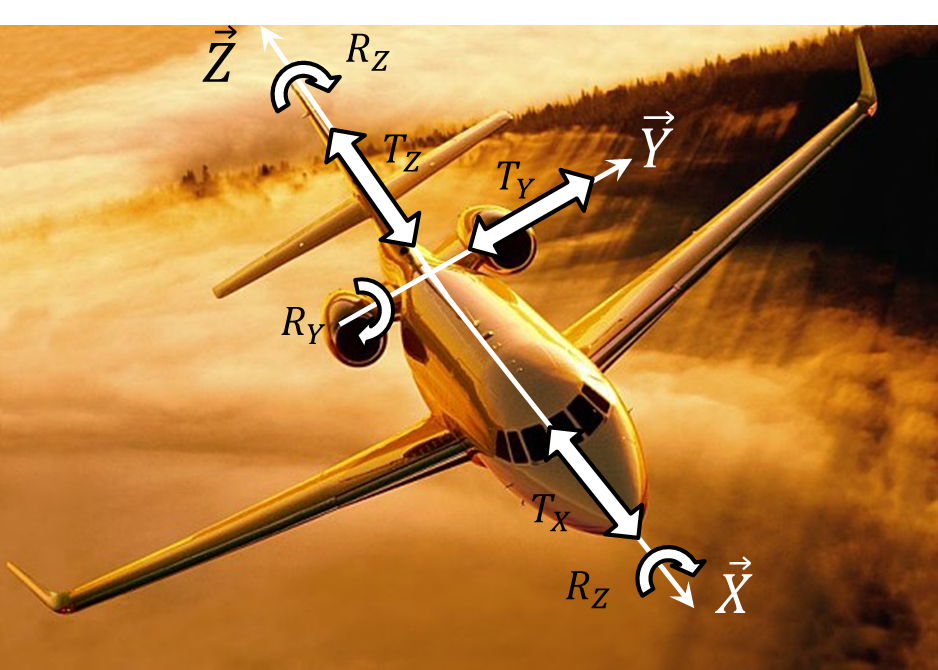
\includegraphics[height=2.5cm]{png/avion}

%\textit{Trainer Solo Sport \cite{cite1}} 
\end{center}
\end{minipage} \hfill
\begin{minipage}[c]{.3\linewidth}
\begin{center}
%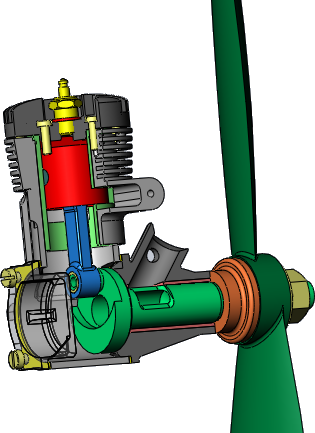
\includegraphics[height=3.5cm]{png/moteur_3d}

%\textit{Modèle CAO d'un moteur de modélisme \cite{cite2}}
\end{center}
\end{minipage} \hfill
\begin{minipage}[c]{.3\linewidth}
\begin{center}
%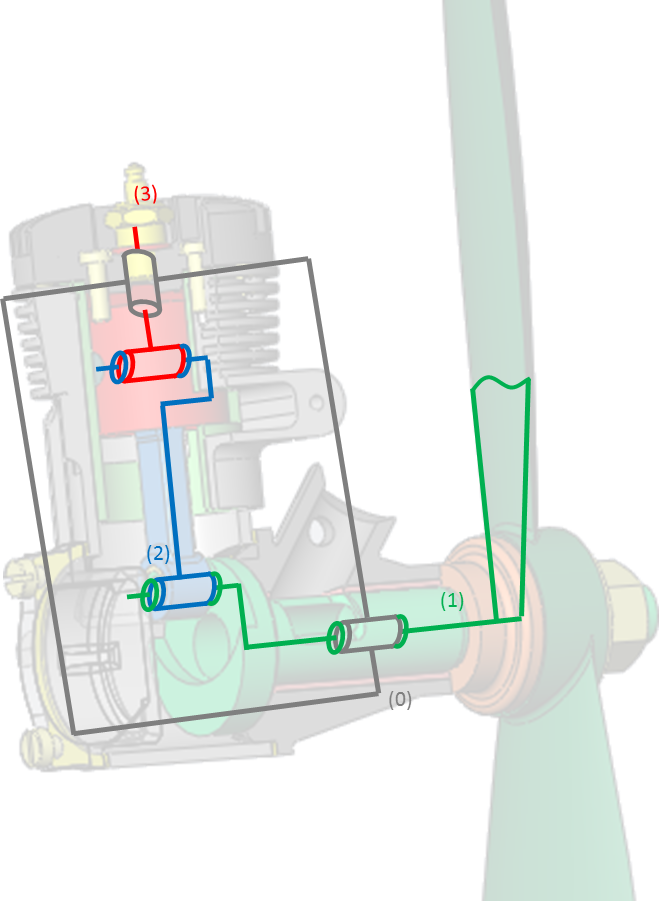
\includegraphics[height=3.5cm]{png/moteur_3d_sch}

%\textit{Modélisation par schéma cinématique}
\end{center}
\end{minipage}


\begin{savoir}
\textbf{Savoirs :}
\begin{itemize}
\item %Rés-C1.1 : Fermeture géométrique.
\end{itemize}
\end{savoir}

\setlength{\parskip}{0ex plus 0.2ex minus 0ex}
 \renewcommand{\contentsname}{}
 \renewcommand{\baselinestretch}{1}



\textit{Ce document est en évolution permanente. Merci de signaler toutes erreurs ou coquilles.}
\tableofcontents

 \renewcommand{\baselinestretch}{1.2}
\setlength{\parskip}{2ex plus 0.5ex minus 0.2ex}



\section{Avant propos}

\subsection{Notion de solide indéformable}
\subsection{Notion de point appartenant à un solide}

\section{Trajectoire d'un point appartenant à un solide}

\section{Vitesse d'un point appartenant à un solide}



\subsection{Définition du vecteur vitesse}

\begin{defi}
\textbf{Vitesse d'un point appartenant à un solide}

Soit un solide $S_0$ auquel on associe le repère $\mathcal{R}_0$ $\left(O_0,\vect{i_0};\vect{j_0},\vect{k_0} \right)$.  Soit un solide $S_1$ auquel on associe le repère $\mathcal{R}_1$,  $\left(O_1,\vect{i_1};\vect{j_1};\vect{k_1} \right)$. Le solide $S_1$ est en mouvement par rapport au solide $S_0$. 

Soit un point $P$ appartenant au solide $S_1$. La vitesse du point $P$ appartenant au solide $S_1$ par rapport au solide $S_0$ se calcule donc ainsi : 
$$
\vect{V(P\in S_1/S_0)}(t) = \left[\dfrac{d\vect{OP(t)}}{dt}\right]_{\mathcal{R}_0}
$$
\end{defi}

\begin{warn}
\begin{minipage}[c]{.15\linewidth}
\begin{center}

\includegraphics[width=.8\textwidth]{png/warning3}
\end{center}
\end{minipage} \hfill
\begin{minipage}[c]{.8\linewidth}
\begin{itemize}
\item Attention à respecter rigoureusement la notation.
\item La vitesse dépend du point d'application.
\end{itemize}
\end{minipage}
\end{warn}


\begin{rem}
\begin{minipage}[c]{.65\linewidth}
Lorsqu'un point est confondu pour deux solides (centre d'une liaison pivot ou d'une liaison rotule par exemple) les vitesses sont égales ainsi, ici : 
$$
\vect{V(0_2\in S_1/S_0)}(t) = \vect{V(0_2\in S_2/S_0)}(t)
$$
\end{minipage}\hfill
\begin{minipage}[c]{.3\linewidth}
\begin{center}
%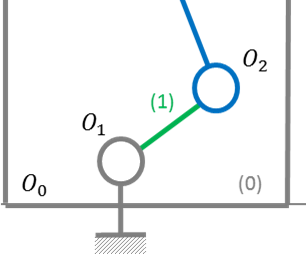
\includegraphics[width=.8\textwidth]{png/2solides}
\end{center}
\end{minipage}
\end{rem}

\begin{rem}
Dérivée d'un vecteur
\end{rem}

\begin{exemple}
\end{exemple}

\subsection{Vecteur instantané de rotation}
Soit un avion $S_1$ repéré par le repère $\mathcal{R}_1\left(O_1,\vect{i_1},\vect{j_1},\vect{k_1} \right)$ en mouvement libre par rapport à un repère $\mathcal{R}_0\left(O_0,\vect{i_0},\vect{j_0},\vect{k_0} \right)$.  La position de l'avion dans l'espace est repéré par le vecteur $\vect{O_0O_1}=x(t)\vect{i_0}+y(t)\vect{j_0}+z(t)\vect{j_0}$ ainsi que par les angles d'Euler.

\begin{minipage}[c]{.65\linewidth}
\begin{center}
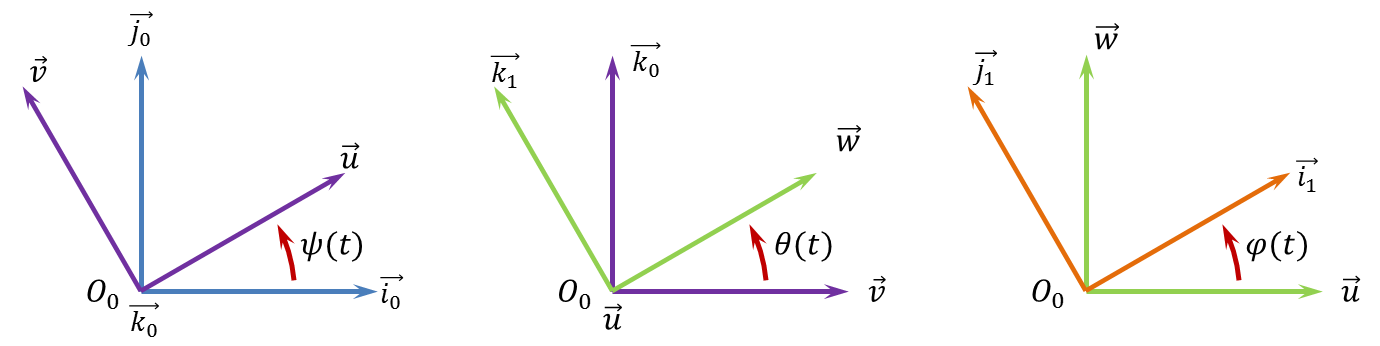
\includegraphics[width=.95\textwidth]{png/euler}
\end{center}
\end{minipage}\hfill
\begin{minipage}[c]{.3\linewidth}
\end{minipage}


Calculons la vitesse du point $O_1$ par rapport à $\mathcal{R}_0$ :
\begin{eqnarray*}
\vectv{O_1}{S_1}{S_0} &=&  \left[\dfrac{d\vect{O_0 O_1}(t)}{dt}\right]_{\mathcal{R}_0} \\
&=& \left[\dfrac{d\left(x(t)\vect{i_0}+y(t)\vect{j_0}+z(t)\vect{j_0} \right)}{dt}\right]_{\mathcal{R}_0}
= 
\left[\dfrac{d\left(x(t)\vect{i_0}\right)}{dt}\right]_{\mathcal{R}_0}
+\left[\dfrac{d\left(y(t)\vect{j_0}\right)}{dt}\right]_{\mathcal{R}_0}
+\left[\dfrac{d\left(z(t)\vect{k_0}\right)}{dt}\right]_{\mathcal{R}_0} \\
&=&
x(t)\underbrace{\left[\dfrac{d\vect{i_0}}{dt}\right]_{\mathcal{R}_0}}_{\vect{0}}
+ \left[\dfrac{dx(t)}{dt}\right]_{\mathcal{R}_0} \vect{i_0}
+y(t)\underbrace{\left[\dfrac{d\vect{j_0}}{dt}\right]_{\mathcal{R}_0}}_{\vect{0}}
+ \left[\dfrac{dy(t)}{dt}\right]_{\mathcal{R}_0} \vect{j_0}
+z(t)\underbrace{\left[\dfrac{d\vect{k_0}}{dt}\right]_{\mathcal{R}_0}}_{\vect{0}} 
+ \left[\dfrac{dz(t)}{dt}\right]_{\mathcal{R}_0} \vect{k_0} \\
&= &\dot{x(t)}\vect{i_0}+\dot{y(t)}\vect{j_0}+\dot{z(t)}\vect{k_0}
\end{eqnarray*}


Soit $P$ un point appartenant à l'avion tel que $\vect{O_1P}=a\vect{i_1}+b\vect{j_1}+c\vect{k_1}$. Calculons la vitesse du point $P$ par rapport à $\mathcal{R}_0$ :

$$
\vectv{P}{S_1}{S_0}=\left[\dfrac{d\vect{O_0 P}(t)}{dt}\right]_{\mathcal{R}_0}
= \left[\dfrac{d\left( \vect{O_0 O_1} + \vect{O_1P}\right)(t)}{dt}\right]_{\mathcal{R}_0}
=\underbrace{\left[\dfrac{d\vect{O_0 O_1}(t)}{dt}\right]_{\mathcal{R}_0}}_{\vectv{O_1}{S_1}{S_0}}
+\left[\dfrac{d\vect{O_1 P}(t)}{dt}\right]_{\mathcal{R}_0}
$$

Calculons donc $\left[\dfrac{d\vect{O_1 P}(t)}{dt}\right]_{\mathcal{R}_0}$ :
\begin{eqnarray*}
\left[\dfrac{d\vect{O_1 P}(t)}{dt}\right]_{\mathcal{R}_0} & = & 
\left[\dfrac{d\left(a\vect{i_1}+b\vect{j_1}+c\vect{j_1} \right)}{dt}\right]_{\mathcal{R}_0} \\
& = & a\left[\dfrac{d\vect{i_1}}{dt}\right]_{\mathcal{R}_0}
+ \underbrace{\left[\dfrac{da}{dt}\right]_{\mathcal{R}_0}}_{\vect{0}} \vect{i_1}
+b\left[\dfrac{d\vect{j_1}}{dt}\right]_{\mathcal{R}_0}
+ \underbrace{\left[\dfrac{db}{dt}\right]_{\mathcal{R}_0}}_{\vect{0}} \vect{j_1}
+c\left[\dfrac{d\vect{k_1}}{dt}\right]_{\mathcal{R}_0} 
+ \underbrace{\left[\dfrac{dc}{dt}\right]_{\mathcal{R}_0}}_{\vect{0}} \vect{k_1} \\
& = & a\left[\dfrac{d\vect{i_1}}{dt}\right]_{\mathcal{R}_0}
+b\left[\dfrac{d\vect{j_1}}{dt}\right]_{\mathcal{R}_0}
+c\left[\dfrac{d\vect{k_1}}{dt}\right]_{\mathcal{R}_0} \\
\end{eqnarray*}

Pour dériver les vecteurs $\vect{i_1}$, $\vect{j_1}$ et $\vect{k_1}$ dans la base $\mathcal{R}_0$ il faut les exprimer dans $\mathcal{R}_0$. On a donc :

\begin{eqnarray*}
\vect{i_1} & = &  \cos\varphi(t) \vect{u} +  \sin\varphi(t) \vect{w}  \\
 & = & \cos\varphi(t)\left(\cos \psi(t) \vect{i_0}+\sin \psi(t) \vect{j_0} \right)+  \sin\varphi(t) \left( \cos \theta(t) \vect{v}+\sin \theta(t) \vect{k_0} \right) \\
 & = & \cos\varphi(t)\left(\cos \psi(t) \vect{i_0}+\sin \psi(t) \vect{j_0} \right)+  \sin\varphi(t) \left( \cos \theta(t) \left(\cos \psi(t) \vect{j_0}-\sin \psi(t) \vect{i_0}  \right)+\sin \theta(t) \vect{k_0} \right) \\
& = & \left(\cos\varphi(t)\cos \psi(t) - \sin\varphi(t) \cos \theta(t)\sin \psi(t) \right)\vect{i_0}  + \left(\cos\varphi(t) \sin \psi(t) + \sin\varphi(t) \cos \theta(t) \cos \psi(t) \right)\vect{j_0} + \sin\varphi(t) \sin \theta(t) \vect{k_0}\\
\vect{j_1} & = & \\
\vect{k_1} & = & \\
\end{eqnarray*}

\subsection{Champ des vecteurs vitesses des points d'un solide}




\section{Accélération d'un point appartenant à un solide}


\begin{thebibliography}{2}
%\bibitem[1]{cite1} Trainer Solo Sport, \textit{Avio et Tiger}, \url{http://www.net-loisirs.com/trainer-solo-sport-p1155.html}.
%\bibitem[2]{cite2} Université Bretagne Sud, \textit{Moteur de modélisme} \url{http://foad.univ-ubs.fr/file.php/1355/TP_meca3d/Moteur_modelisme.zip}.
%\bibitem[3]{JPP} Jean-Pierre Pupier -- Paramétrage -- PTSI -- Lycée Rouvière Toulon.
\end{thebibliography}
\end{document}

